%*****************************************
\chapter{Literature Review}\label{ch:examples}
%*****************************************
\section{Automation and Human Agent interaction}
The study Automation design and Human agent interaction are two heavily intersected research areas which overarches this PhD work.  


\subsection{A History of Automation }
The original goal of Automation is to replace the tasks originally performed by human with a machine. \cite{Bradshaw2011} . It can be defined as the execution by machine, usually computer, of a function previously performed by human [Parasuraman and Riley 1997] The tasks that can be automated is used to be limited by technical capabilities, but this is no longer the case. With quick growth of machine's speed and intelligence, the tasks that can be automated is rapidly increasing, including complex cognitive activities such as information analysis, planning and decision making.[RAJA] The boundary between human machine capabilities has blurred. With little cannot be automated, the automation designers have to make hard choice about what to automate and to what extent.\\

One traditional approach for automation design is to simply automate all system functions that can be automated easily in a cost-effective way, leaving the all remaining tasks to human operators. The main considerations in this approach are technical capability and cost. The assumption of this approach is that the automation of sub systems functions can lead to optimisation of whole system with no detrimental impact results from the automation. However this is not always the case, Large body of empirical work in automation design have shown that xxxx .\\ 

The other approach is to achieve division of labour between human and automation according to their strength and weakness. As in Fitts list \cite{Fitts} , a set of strengths and weaknesses of humans and machines is identified. Some study pointed the division of labour would not be as simple as a labour division according to strength and weakness[]. Firstly the time factor could be important because human and machine's availability may change overtime. Secondly By delegating the same task to machine, the nature of human tasks can be changed as well. Large body of work has shown clearly that automation does not simply supplant human activity but rather changes it, often in a way that is unanticipated by the system designer. [Coordination and Supervision interaction required, expand ] \cite{Bradshaw2011} [Later , proposed by Licklider in the un-Fitts list \cite{Hoffman2002}, automation is aimed to leverage and extent human capability by using agents (not replacing).\cite{Bradshaw2011}.] \\


\subsection{The Level of Automation}
More recently, another alternative model of automation to guide automation design is proposed by proposed by C. D. Wickens[],known as 10 level model of automation. The model 10 levels of automation (LOA) has been later extended by R Parasuraman [] with more detailed classification of automation types. The extended model of LOA informs study approach of this PhD work, which will be documented in chapter x. This section will give an introduction of this model. 


Most tasks can be fully or partially automated, which implies that automation is not all or none, but can vary across a continuum of level[]. At the lowest level, all system functions are performed manually by human operators.  At highest level, system are fully automated, taking over all system functions. In between this two extremes, 10 different levels of automation are proposed by xxx. As shown in table x. 


\subsection{Definition of Software Agent }

Since creation of the term "software agent", there are a lot of debates about its definition . One definition commonly shared by the Multi-Agent system(MAS) literatures is that the software agents are designed to operate independently without constant human supervision. In the AI community, the software agent evolves from multi-agent system research which in turn, derived from the field of Distributed AI \cite{Vlassis2007}. This strand of work investigates infrastructure, language and communication to realize coordinated agent software system. The goal was to specify, analyse, design and integrate systems comprising of multiple collaborative agents.\cite{Nwana1996} \\

More recently, the use of the word software agent become much more diversified. \cite{Nwana1996} has made attempts to investigate broader classes and types of agent. Nwana's \cite{Nwana1996} topology of agents identified three characteristics of agents, learning, autonmous and collabroitive, Based on this characteristics, software agents can be categorised into 8 classes, rangin g from collaboration agents, information agents to interface agents. \\

With a broader definition, researchers begin to investigate broader issues surrounding development of agent systems, among which human agent interactions have attracted a lot of attention of researchers and practitioners.[get one reference here!!!]

\subsection{Human Agent Interactions }

Automation design and Human agent interactions have big overlaps as both concerns the impact of automation(by computational systems) on human performance. While automation design is trying to answer the question of what and to what extent the automation should be, the study of human agent interaction concerns the issue of interaction design related to development of human agent system, with the aim to develop agents which is good at teamworking with human operators. 

The agent researchers adopted a view that human and agents are equally important team players in a human agent system.[] It highlights the importance of mutual interaction between human and agents that can enhance the competencies of both human and systems. From this perspective, the aim of automation is no longer "replace" human but achieve an human-machine symbiosis through effective human agent coordination, which is similar to the view adopted by xxx in developing un-fitts list. As researchers realize the effective human-machine symbiosis requires sophisticated interactions design between human and agent, the "interactional" issues of automation is thought to be as important as technical issues.[Expand discussion about this issues.] \cite{Bradshaw2011} \\

Several interaction techniques have been devised by agent researchers to achieve effective coordination between human and agent. [expand on mixed initiative and flexible autonomy]

[define the interactional issues!!!!]

\subsection{Human agent collectives}


\subsection{Issues in Human Agent Interactions }
Combine both 

Why the social issues of designing agent system is important? [Norman1994]
state lesson from CSCW



\subsection{Summary}

Because this PhD work sits in the overlapping research area of human agent interaction and automation design, the later chapters will consider automation and agent software as two interchangeable concepts.

\section{Task Planning in Disaster Response}\label{sec:lrplanning}
To define a context of task planning activities in disaster response, This section begins with a definition of disaster response, followed by an overview of command and control structures of DR organisation which facilitates task planning. The final section (\ref{sec:LRtaskplanning}) examines the main characteristics of task planning in DR.


\subsection{Define disaster response}
There are no standardized rules defining the different phases of the disaster management. Different countries and agencies may apply different rules and standards, but most of them agreed the disaster management is carried out in a circle. Figure 5 illustrates the a model of disaster management cycle described in the literature \cite{Wattegama2012} :\\

%insert picture

\begin{enumerate}
\item Mitigation: any activity that reduces either the chance of a hazard taking place or a hazard turning into disaster.
\item Risk reduction: anticipatory measures and actions that seek to avoid future risks as a result of a disaster.
\item Prevention: avoiding a disaster even at the eleventh hour. 
\item Preparedness: plans or preparations made to save lives or property,and help the response and rescue service operations. This phase covers implementation/operation, early warning systems and capacity building so the population will react appropriately when an early warning is issued.
\item Response: includes actions taken to save lives and prevent property damage, and to preserve the environment during emergencies or disasters. The response phase is the implementation of action plans.
\item Recovery: includes actions that assist a community to return to a sense of normalcy after a disaster.
\end{enumerate}

The disaster response operations refer to the actions taken during or immediate aftermath of the disaster strike. In this period, a significant number of individuals may be trapped and injured. Great number of structural damages need be dealt with. Medicine, food and shelters are in great demand. This period calls for prompt action within an exceptionally short period of time \cite{Wattegama2012}. Responder team may find themselves with limited resources and need to make plans to utilities the resources in a timely and satisfactory manner \cite{Chen2005,Chen2008}. \\

%\subsection{Team coordination in disaster response}
%Malone (1990 361) defines coordination as the act of managing interdependencies between activities performed to achieve a goal. One of the very important component of coordination in DR, following sections will firstly... and then discuss how the coordination is carried out through command structure of DR team. \\

%In disaster response, team coordination is essential in order that groups of people can carry out interdependent activities together in a timely and satisfactory manner (cf. Bradshaw et al., 2011). Disaster response experts report that failures in team coordination are the most significant factor in critical emergency response (Toups et al., 2011: 2) that can cost human lives. Shared understanding, situation awareness, and alignment of cooperative action through on-going communication are key requirements to enable successful coordination. Convertino et al. (2011) design and study a set of tools to support common ground and aware- ness in emergency management. \\

\subsection{DR command structure}
The emergency response agencies typically employs a hierarchical command structure \cite{Ramchurn}. One widely used command and control structure the Gold, Silver, Bronze model. In this model, decision making is divided into strategic, tactical, and operational levels. The teams responsible for each are referred to as Gold, Silver, and Bronze respectively. The decisions on main objectives of the response effort are made at the strategic (Gold) level. At the tactical level, based on the specified objectives, the Silver command team decides on the allocation of resources and tasks to be carried out, while at the operational level, Bronze first responders (FRs), on the ground, determine the logistics required to carry out those tasks. Information gathered from the ground is also passed back up from Bronze, through Silver, to Gold.\\

Some literatures \cite{Chen2005,Chen2008} also generalized the command and control structures as a generic two level model. The key characteristic of the two-level model is division between remote coordination center and on site teams.  On-site responders react to immediate scene without global picture, while the coordination center deals with strategic issues and works with a global picture, leveraging external resources to help on-site response. \\

%insert picture 

\subsection{Task planning in large scale disaster} \label{sec:LRtaskplanning}
One important characteristic of large-scale disaster is the presence of multiple spatially distributed incidents \cite{Chen2005}. To gain insight into the problem of task and resource allocation in large scale disaster, we will firstly examine how a single incident is dealt with. The procedures of dealing with single emergency incident have documented by a number of field studies \cite{Comfort2004,Dawes2004,Petrescu-prahova2005}. In Toups's \cite{Toups2011} study, fire emergency response to small-scale structural fires is depicted as follow: 

\begin{quote}
Fire emergency response is undertaken by small teams distributed throughout the incident, coordinated by an incident commander (IC) . Multiple response teams, or companies, are dispatched to any incident and cooperate around the fireground. A company officer leads each team, which consists of firefighters and/or engineers.2 Normally, each company is associated with a firefighting vehicle; an apparatus, such as an ambulance, engine, or ladder truck.\\
\end{quote}

For the depiction of single incident emergency response, we can see a combination of different resources (e.g. ambulance, fire engine, ladder truck ) and skills (e.g. structural engineers, firefighters and medics) need to deployed to the location of the incident. To deal with multiple incidents, the disaster response team has to coordinate spatially distributed resources and personnel to carry out operations (e.g. search, rescue and evacuation)\cite{Chen2005}. That is , resources and responders needed to by divided and combined in to teams and deployed to handle distributed incidents. Depending on the number of incidents, response personnel may need to dispatch, deploy and redeploy limited resources. One major concern for task planning in disaster response is how to efficiently allocate limited resources to multiple incidents with temporal and spatial constraints \cite{Bradshaw2011}.\\

The task environment of DR is characterised by various uncertainties including hazard uncertainties, task-flow uncertainties, environmental and informational uncertainties \cite{Chen2008}. Sudden and unexpected events may occur as the disaster situation unfolds. Therefore, fixed plans of actions for responders is unlikely to work. The uncertainties may need to be handled by improvisation, prioritisation, and dynamic sourcing of capabilities \cite{Faraj2006}, which means dynamic change of plans is necessary to deal with uncertainties in dynamic task environment.\\    


%geo-distribution and time pressure has been identified as challenges for task planning and execution. Uncertainty new means real time and dynamic task planning[chen's emergency response]. Geo distribution creates uncertain in the information [short distributed team paper][the human factor in dr paper discussion failure of communication] and creates time constraint as well because teams need to be  \\


%chen's emergency response some practitioners articles

%The fireground and surrounding space constitute a dangerous and dynamic interface ecosystem [Kerne 2005] of distributed cognition, connecting responders, victims, fire- fighting equipment, communication media, and information artifacts. Upon arriving at an incident, multiple companies distribute in and around the fireground. Compa- nies and their apparatuses are placed at strategic locations, and are moved as needed. Human operators work on and from these platforms. Firefighters and rescue workers deploy from them, taking equipment into the fireground; equipment, such as firehoses and radios, may be technologically supported by the apparatus itself (pumps and water sources, or high-power repeaters, respectively). Each apparatus, and in many cases, each human worker, is equipped with a half-duplex radio to facilitate long-range, broad- cast communication.\\

\section{Technology support for task planning}
Technology support systems designed for planning is unlikely to be an isolated computational entity. It is better to be seen as `toolbox' that contains various connected components \cite{Wattegama2012}. To give an overview of current technological practices related planning support, This section will review three related research domains with the context of computational DR support - Task planning systems for plan formulation and evaluation ; the Information and communication technologies (ICT) for information acquisition and management; and the AI(Artificial intelligence) based technologies for disaster simulation, and task optimisation. The section \ref{sec:lraisupport} also will examine how the agent-based planning support system to be studied in this PhD study can be positioned with respect to the three research domains. \\

\subsection{Planning support systems}
%spatial and time constraint
The planning support system (PPS) can be defined as a suite of components that help planners to explore and manage planning activities \cite{Geertman2004}.Literatures have documented a variety of planning support system with a range of purposes such as land development[], logistic scheduling[],and evacuation planning[]. This section will further refine the scope of planning support systems according to some key characteristics of disaster response(DR) operations identified in section x.

In the context of disaster response, planning activities  typically concern dispatch, routing and deployment of rescue resources (see section \ref{sec:LRtaskplanning}). Therefore, we consider the geo-information tools/systems (GIS) for spatial analysis may be a central component of planning support suite. While the general-purpose GIS  are only designed to handle geo-spatial data \cite{Geertman2004}, the planning support system consists of a wide variety of functionalities to support multiple aspects of planning process, which may include, but not limited to problem diagnosis, data collection, mining and extraction, data modelling, visualisation and display, scenario-building and projection, plan formulation and evaluation, and collaborative decision-making support \cite{Geertman2004}. \\

The time-critical task setting may be another major factor that makes a DR planning system differs from others. In disaster response operations, responders (as planners) may need to plan dynamically according to the disaster environment are always quickly changing. Once we extend the capabilities planning system with real-time capabilities, the boundary between planning system and command/control systems (e.g ground traffic and aviation control) are blurred. In this PhD work, we will call the system sittings in the middle ground area `real time planning' system.\\

Some researches treat command and control system as automation tools aspects of command control activities including information acquisition, analysis, decision selection and action implementation[underground paper].  In contrast, a `real-time planning support system' may have stronger focus on supporting real-time plan generation and decision selection. In the domain of disaster response, efforts have been made to study and design such real-time task planning system for DR \cite{Wagner2004,Okaya}, but the real deployments are still rare.\\

\subsection{ICT support for disaster response}
The information and communication technology support (ICT) includes communication infrastructures and software system on top of the infrastructures. The communication infrastructures refer to communication channels including radio, television, satellite, internet, text and voice communication over mobile phone. The basic communication infrastructures have long be utilised by responders to capture both soft data (generated by human) and hard data (from sensors) for their decision making \cite{Fischer2012}. Apart from the infrastructures, the ICT are  software systems are playing increasingly important role. Now days, most DR practice may consists  of both the manual processes which direct utilize ICT infrastructures and the use of ICT software for data analysis and information management. The figure \ref{fig:ICTExample} illustrate a tsunami response system operated by Asian Disaster Preparedness Center(ADPC). The technical components are comprised of a network of seismographic stations, sea-level gauges and deep-sea pressure sensors. A data-processing and tsunami forecasting centre is equipped with seismic processing and modelling software.  Tsunami warnings are disseminated through the communication links between national centres and the people at risk, which includes, email, television, radio, cellphones and satellites.\\

\begin{figure}[h]
  \centering
  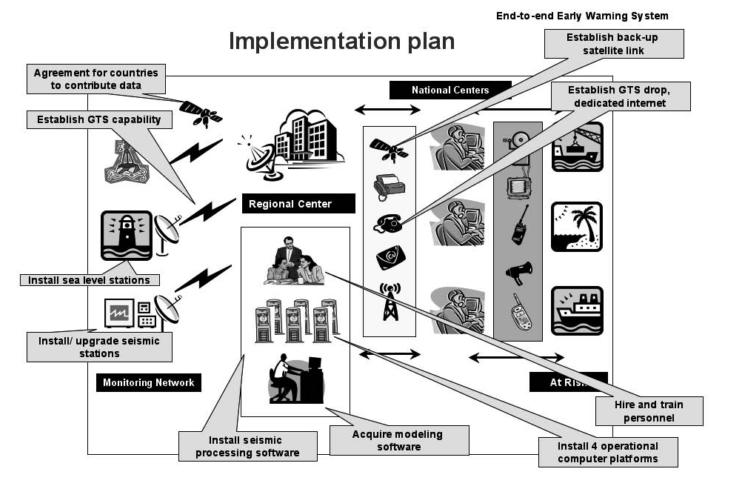
\includegraphics[width=1\textwidth]{img/background/ICTExample}
  \caption{Tsunami response system}
  \label{fig:ICTExample}
\end{figure}

With proliferation of smart phones and ubiquitous computing technologies, internet have become increasingly important in the disaster response. Web-based applications have been used in the indian ocean tsunami for tracking missing people, coordinating donors, and recording locations of shelters \cite{Wattegama2012}. The possibilities for public participation are expanding with increased access to the Internet and the wide diffusion of mobile technology. For example, some wiki style websites are used in recent disaster. With utilities of such websites, the public is able to take not only a more active part in seeking information, but also in providing information to each other, as well as to formal response efforts \cite{Palen2007}.\\

From the author's point of view, a task planning support must heavily rely on ICT infrastructure for data acquisition and plan implementation. Functionalities of ICT software may also have many overlaps with that of task planning systems, in the sense that they all support responders to acquire, process and manage information for the use of decision making in DR. \\


\subsection{Application of AI technologies}\label{sec:lraisupport}
In the field of AI, machine learning and agent-based algorithms have increased in availability for disaster response. The AI technologies such as agent-based disaster simulations \cite{Okaya} have long been utilised by us to understand and prepare for disasters. With the increase in the networked computers, sensors and amount of data generated from different sources in real time \cite{Ramchurn}, there are increasing demand for intelligent computational support for data processing and task planning. Researchers from ORCHID project have developed a prototype system - HAC-ER (Human Agent Collectives for Emergence Response), which demonstrates how the AI algorithms may transform the landscape of real time task planning in DR.\\

The HAC-ER system consists of a set of connected components for real-time task planning support, each of which are powered by multiple machine learning and agent-based algorithms. First, a component called Crowedscanner is used to deal with vast quantities of unstructured data produced very rapidly on the internet as disaster unfolds, such as text messages or photographs from web-based platforms such as Twitter or Ushahidi[]. The approach is to use a machine learning algorithms (for details, see IBCC []) to fuses heterogeneous reports from both into unreliable and trusted sources a common picture of the disaster, or a heatmap of incidents. Second, multiple  UAVs (Unmanned Aerial Vehicles) is deployed as mobile sensors to search or further inspect incidents reported by crowdscanner. The control of multiple UAVs is assisted by multi-agent coordination algorithm (Max-sum \cite{Ramchurn2010}). The algorithm is capable of quickly optimise the task allocation for UAVs to visit points of interest or conduct search in an area.  Finally, responders and assets on the ground will need to be dispatched and deployed to deal with distributed incidents. Another HAC-ER component is designed to assist human operators in the control room to conduct real-time planning. The component is powered by a coordination algorithm based on MMDP modelling techniques [Feng's MMDP paper]. Taking into to account the priorities of incidents, and locations of responders teams and incidents, the algorithm can produces computationally optimised task allocations for responder teams to attend as many incidents as possible with a time constraint. Further, algorithms and interfaces of all components in HAC-ER are designed in a way that accept human input. The HAC-ER depicted a picture in which human operators and intelligent components collaboratively conduct task planning. The picture demonstrates the potential for applying AI in DR task planning.\\

\subsection{Summary}
This section have reviewed technological practices related to planning support in disaster response. First, there are great deal of GIS-enabled planning support systems (PPS), the planning system with real time support is rare in the disaster response domain. Second, the ICT infrastructures and softwares have long be utilised by responders for managing communication and information. The author believe ICT provides basis for real-time task in the sense that it provide functionalities to support information acquisition and management. Finally, AI researcher have devised some machine learning and agent-based algorithms to support task planning. Prototype systems have been built to demonstrate the potential for planning support based on AI technologies. \\

So far, we have framed the problem of task planning in DR (section x) and reviewed three research domains related building planning system to support task planning in this section. It should be emphasised that this PhD work is primarily interested in a real-time task planning system that utilise ICT technologies as its underlying infrastructures and is based on intelligent coordination algorithms. And this kind of system can be located in the overlapping area of the three research domains that is reviewed in this section (see figure x).

%insert figure 

\section{A CSCW perspective to technology support}



\section{Game based simulation} \label{sec:LRMRgame}
This PhD work adopts serious mixed reality game approach to investigate the issues of interaction surrounding agent planning support for disaster response operations. This section will firstly go through aome literatures of serious games to give an overview of history and applications areas of serious games. Then, mixed reality game (MRG) will be introduced, followed by discussion of the potential for using MRGs to support ethnographic study of ubiquitous systems, which underpins the rationale of serious MRG approach applied in this PhD study.\\ 


%COOP
%We adopt a serious mixed-reality games approach to create a setting in which participants experience physical exertion and stress through bodily activity and time pressure, mirroring aspects of a real disaster setting (PAHO, 2001). We use game probes as a complementary approach to gathering system requirements for real-world settings, for example in addition to co-designing with users. Our game probe explores a socio-technical setting in which field responders receive guidance from a central command headquarters (‘HQ’), inspired by the concept of the Sector Coordinator in USAR task forces (INSARAG, 2012). \\
%Computational simulations, particularly agent-based simulations of disasters, are the predominant approach in the computing literature to predict the consequences of “courses of action” (Hawe et al., 2012), e.g., to model first responder information flow (Robinson and Brown, 2005), or logistic distribution of emergency relief supplies (Lee et al., 2007). \\

%Limitations of the veracity of computational simulations are manifold. For ex-ample, Simonovic highlights that simulations may rely on unrealistic geographical topography, and most importantly, may not account for “human psychosocial characteristics and individual movement, and (…) learning ability” (Simonovic, 2009: 89). The impact of emotional and physical responses likely in a disaster, such as stress, fear, exertion or panic (Drury et al., 2009) remains underaddressed in approaches that rely purely on computational simulation. 
%One of our work’s main objectives is to study interaction and coordination sit-uated in rich and ‘messy’ real-world socio-technical settings. As it is difficult to deploy technological prototypes in real disasters, game-like simulations have been adopted to study technology interaction in disaster scenarios, for example to pre-pare first responders for scenarios in which hazardous materials are involved (Losh, 2007). Abbasi et al. (2012) present a study in which locally distributed par-ticipants played the role of victims asking for help via social media in a simulated crisis, and participants that played the role of first responders used a coordination system to filter messages and mobilize the appropriate responder teams according to their assigned capabilities. Toups, Kerne and Hamilton (2011) present the de-sign and evaluation of the Team Coordination Game, which teaches participants effective cooperation and – in particular – communication, based on a zero-fidelity simulation of team coordination that focuses on distributed cognition in lieu of concrete details, yet draws directly from fire emergency response work practice.\\

%We adopt a serious-mixed reality games approach (Fischer et al., 2012) to cre-ate a game probe that enables studying team coordination, interaction and com-munication in a real-world disaster scenario whilst providing confidence in the ef-ficacy of behavioural observations. Suspension of disbelief occurs frequently in the play of pervasive or mixed-reality games (Stenros et al., 2009). Mixed-reality games bridge the physical and the digital (Benford et al., 2005). They serve as a vehicle to study distributed interactions across multiple devices and ubiquitous computing environments ‘in the wild’ (Crabtree et al., 2006). \\
%One important characteristic of large-scale disaster is the presence of multiple spatially distributed incidents (Chen et al., 2005). To deal with multiple incidents, the disaster response team has to coordinate spatially distributed resources and personnel to carry out operations (e.g. search, rescue and evacuation). 
%Depending on the proliferation of incidents, response personnel may need to dispatch, deploy and redeploy limited resources. Coordination is required to effi-ciently allocate limited resources to multiple incidents with temporal and spatial constraints imposed by the nature of disasters. \\

%Mixed-reality games (MRG) share a common set of characteristics with time critical settings, such as disaster response (DR):
%Bridging the physical and the digital. Both DR as well as MRGs routinely bridge the physical and the digital as part of their actors’ coordination (Benford et al., 2005). DR for example makes use of the twitterverse to inform real world response (e.g., Sarcevic et al., 2012).

%Orchestration. DR and MRGs are both highly orchestrated activities. Author-ing and orchestration tools `behind the scenes' of an MRG, as well as player in-terfaces, provide managers, players and spectators with different temporal and spatial views of the game world in order to support the experience (Crabtree et al., 2004). These settings are surprisingly comparable to the `control room' of a disaster response operation, in their collections of sophisticated technological arrangements to communicate and coordinate real-time information streams, in order to create a holistic view amidst an immersive setting of interest.\\
%On-the-ground and online. In both DR, as well as in MRGs, people on the ground often work with people online to solve a common problem. Sarcevic et al. (2012) show how understanding online content can foster understanding of medical coordination challenges in DR on the ground. MRGs often leverage the fact that people on the ground and online have different views of the world, which are turned into different abilities within the game (Flintham et al., 2003).\\ 
%These key characteristics illustrate the overlap between time-critical coordina-tion in MRGs and DR. This perspective underlies our motivation to explore the approach of studying team coordination through a game probe.\\



%=========
%Computational simulations are likely to be insufficient in elucidating the social and interactional issues around agent-based coordination support [18]. Therefore we adopt a mixed-reality game approach to put people under realistic cognitive and physical stress. Mixed-reality games are recreational experiences that make use of pervasive technologies such as smart phones, wireless technologies and sensors with the aim of blending game events into a real world environment [6]. Arguably, they have become an established vehicle to explore socio-technical issues in complex real world settings [5]. The major advantage of mixed-reality games is the fact that they are situated in the real world, which arguably leads to increased efficacy of the behavioural observations when compared to computational simulations. 
%

\subsection{Serious Game}
% []

There are various definitions for the term `serious game' in literatures. One issue that most of the literatures agreed on about `serious game' is that the term is concerned with the use of games and gaming technology for the purposes other then mere entertainment, such as education, training, healthcare, and advertisement. Although serious games usually have looks and feels of digital games, they are actually simulations of real-world events or processes. by engaging the participants with simulated environments and systems, the serious games allow learners to experience situations that are impossible in the real world for reasons of safety, cost, time, etc. (Corti, 2006; Squire and Jenkins, 2003). \\

Recently, the serious games have increasingly been applied in the area of disaster response. In particular, 'serious games' are developed for training and simulation of terrorist attacks, disease outbreaks, biohazards, traffic control and fire fighting etc (Michael and Chen, 2006; Squire and Jenkins, 2003). \\

One good example of serious game for disaster response(DR) is the Biohazard developed by MIT Comparative Media Studies. The video game is designed to help emergency first responders deal with toxic spills in public locations. Emergency responders work in teams to organize the response to a gas attack in a crowded suburban shopping mall. The game objective is to save as many civilians as possible with a time constant. In the game,  players need to quickly assess the situation, divide into teams, and coordinate with each other to identify source of chemical spill. Players can thus practice recognizing the signs of different chemicals and viruses, examining victims' symptoms, and observing pattern of chemicals spread in differing enviromental conditions.\\

%insert figure

Another example of DR serious game could be the team coordination game developed by Toups, Kerne and Hamilton (2011), which teaches participants effective cooperation and in particular communication, based on a zero-fidelity simulation of team coordination that focuses on distributed cognition in lieu of concrete details, yet draws directly from fire emergency response work practice[]. User study and evaluation of the coordination game have suggested that the a serious game built with low fidelity approach can still help responders to improve there coordination skills.\\

The advantage of serious games in disaster response domain may be obvious. Creating high fidelity excises for disaster response could be costly and dangerous, while the serious games allow participants to repetitively practice without danger and high cost. For instance, the game Biohazard enable players to experiment with a multitude of different conditions and strategies with simple change of some game variables.\\

However, there are also concerns that the existing serious games often fails to capture the social aspects of DR operations. For example, it is argued that the game Biohazard failed to capture complexity of victims behaviour in highly stressful, emergency situations. Therefore, the game may not be able to help responders to develop interpersonal skill (expressed through voice, gestures) which are required to deal with panicked victims[]. In fact, the serious games are usually not designed to simulate all aspects of DR operations, but only to mirror some aspects of DR practices and processes (e.g. zero fidelity coordination game). Serious games are thus not a replacement for field trials and other training methods, but a tool responders can use to explore ideas and talk about their practice.\\

%limitation. People can be unpredictable, particularly in highly stressful, emergency situations. Dealing with a panicked public demands a type of interpersonal skill expressed through voice, gestures, and demean or that contemporary game interfaces cannot capture. Despite the many advances in artificial intelligence in games, characters still can't express a full range of emotional responses in dynamic reaction to events. Clearly, Biohazard is no replacement for experience or even field trials and manuals. Rather, it is a tool that responders can use to explore ideas and talk about their practice. [paraphase] ----- people in DR can be , the game based simulation may fail to simulate panicked public demands and emotional human response. Therefore, the game may not be enough for training of  the human and social aspects of DR domain. Therefore

\subsection{Mixed Reality Games}
Mixed-reality games are one type of digital game which tries to bridge the physical and the digital (Benford et al., 2005) would. The term `mixed reality' refers to virtual experiences being played out in real-world spaces. This kind of games typically use pervasive technologies, such as cellular phones, GPS, Bluetooth, wireless network and sensors, with the aim to blend virtual game events into people's life and real world environment. Some researchers have recognised the potential to adapt mixed reality games for training purposes in Disaster Response (DR) domains [], as the mixed reality game is thought to be a powerful way of exposing participants to learning experiences not otherwise possible. \\

Arguably, the mixed reality game is also becoming an established vehicle to study distributed interactions across multiple devices and ubiquitous computing environments `in the wild' (Crabtree et al., 2006) [Benford, ][me]. The emergence of ubiquitous computing features distributed interaction across a burgeoning array of small, mobile devices and online environments. The mixed reality game also create such an ubiquitous computing environment. Therefore, the mixed reality game can serve as research `probes' for ethnographer and system designer to investigate issues of distributed interactions in the future ubiquitous computing systems.\\

Further, some literatures [] also fund future DR support systems potentially shares a set of characteristics with mixed reality games, which suggests mixed reality game could be a platform for investigating issues of interactions in the DR setting:\\

\begin{enumerate}
\item Bridging the physical and the digital. Both DR as well as MRGs routinely bridge the physical and the digital as part of their actors` coordination (Benford et al., 2005). DR for example makes use of the twitterverse to inform real world response (e.g., Sarcevic et al., 2012).

\item Orchestration. DR and MRGs are both highly orchestrated activities. Author-ing and orchestration tools `behind the scenes' of an MRG, as well as player in-terfaces, provide managers, players and spectators with different temporal and spatial views of the game world in order to support the experience (Crabtree et al., 2004). These settings are surprisingly comparable to the `control room' of a disaster response operation, in their collections of sophisticated technological arrangements to communicate and coordinate real-time information streams, in order to create a holistic view amidst an immersive setting of interest.\\

\item On-the-ground and online. In both DR, as well as in MRGs, people on the ground often work with people online to solve a common problem. Sarcevic et al. (2012) show how understanding online content can foster understanding of medical coordination challenges in DR on the ground. MRGs often leverage the fact that people on the ground and online have different views of the world, which are turned into different abilities within the game (Flintham et al., 2003).\\ 

\item These key characteristics illustrate the overlap between time-critical coordina-tion in MRGs and DR. This perspective underlies our motivation to explore the approach of studying team coordination through a game probe.\\

\end{enumerate}

These key characteristics illustrate the overlap between time-critical, distributed coordination in mixed reality game and DR operation, which makes the mixed reality game ideal platform for investigating potential issues of interactions in future DR support systems.[]\\

%The emergence of ubiquitous computing raises new challenges for ethnography however, distributing interaction across a burgeoning array of small, mobile devices and online environments which exploit invisible sensing systems. Understanding interaction requires ethnographers to reconcile interactions that are, for example, distributed across devices on the street with online interactions in order to assemble coherent understandings of the social character and purchase of ubiquitous computing systems. We


%Mixed-reality games bridge the physical and the digital (Benford et al., 2005). 

%Ubiquitous gaming is one of the most exciting ideas to emerge from the games industry in recent years. Ubiquitous games can be played anytime, anywhere and often play out across multiple media. For example, Electronic Arts' Majestic uses cell phones, desktop computers, and fax machines (among other technologies) to immerse players in a multiplayer conspiracy theory game. Such games motivate players to investigate, weigh evidence, compare notes, test hypothesis, and synthesize information as they draw conclusions about what has occurred and why. We use the terms enhanced reality or augmented reality to refer to virtual experiences being played out in real-world spaces. While such game experiences may seem prohibitively expensive, recent handheld technologies, which can now combine cellular phone, GPS, Bluetooth, wireless Internet, multimedia capabilities, and infrared technologies into one machine, make such experiences possible even on the level of an individual school.\\


%*****************************************
%*****************************************
%*****************************************
%*****************************************
%*****************************************
